\documentclass[a4paper]{article}
\usepackage[pdftex]{graphicx}
\usepackage[utf8]{inputenc}
\usepackage{enumerate}
\usepackage{icomma}
\usepackage{siunitx}
\sisetup{locale=DE}
\usepackage{amssymb}
\usepackage{tikz}
\usepackage{href-ul}
\hypersetup{
	colorlinks=true,
	linkcolor=blue,
	urlcolor=blue}
\usepackage{geometry}
\geometry{a4paper, top=15mm, left=15mm, right=15mm, bottom=15mm,
	headsep=10mm, footskip=12mm}

\begin{document}
	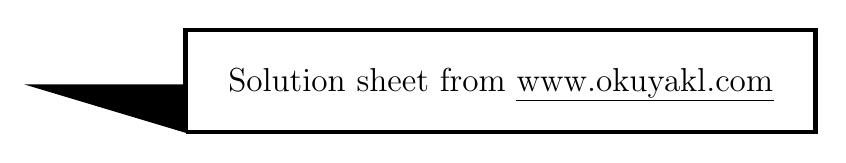
\begin{tikzpicture}(10,3)
		\draw[ultra thick](2,0) --(10,0) -- (10,1.3) --(2,1.3) -- (2,0);
		\draw[fill=black](2,0)-- (0,.6) -- (2,.6) -- (2,0);
		\node at (6,.6) {\large Solution sheet from \href{http://www.okuyakl.com}{www.okuyakl.com}};
	\end{tikzpicture}
	\vspace{0.5 cm}
	
	\noindent
	\begin{minipage}{0.5\textwidth}
		\noindent{\bf Task 1. a)}\\
		\includegraphics[width=7 cm]{gsdrei041}
	\end{minipage}
	\hfill
	\begin{minipage}{0.5\textwidth}
		\noindent{\bf Task 1. b)}\\
		The triangle is isosceles if: $\overline{AC}=\overline{BC}$
		$$
		\renewcommand{\arraystretch}{2}
		\begin{array}{rcll}
			\sqrt{(7-1)^2 + (4-1)^2} &=& \sqrt{(7-10)^2+(4+2)^2} \\
			\sqrt{6^2 + 3^2} &=& \sqrt {3^2+6^2} &(w)\\
		\end{array}
		$$
	\end{minipage}
	
	\noindent{\bf Task 1. c)}\\
	First you calculate the midpoints of two sides of the triangle.
	With this we define two straight lines perpendicular to the respective side.
	We set both line terms equal and get the intersection point $M$. This is the center of the circumference.
	
	\noindent{\bf Task 1. d)}\\
	We consider the route length $\overline{MA}$:
	$$r = \overline{MA}= \sqrt{(5.5-1)^2 + (-0.5-1)^2}=\sqrt{4.5^2 + 1.5^2} =4.74~{\rm LE}$$
	
	\noindent{\bf Task 1. e)}\\
	The area of the triangle is:
	$$ A_D = {1 \over 2}\cdot \left| \begin{array}{cc} 6 & -3 \\ 3 & 6 \end{array} \right|= {1 \over 2} \cdot (36 + 9) = 22.5~{\rm FE}$$
	The area of the perimeter is:
	$$A_k = \pi \cdot r^2 = \pi \cdot 4.74^2 = 70.7~{\rm FE} $$
	The factor is:
	$$ a = {70.7 \over 22.5}=3.14 = \pi $$
	
	\noindent{\bf Task 2.}\\
	\begin{enumerate}[a)]
		\item is false, then $0<k<1$
		\item correct
		\item correct
		\item is wrong because it is only true to the angle but not to the length.
	\end{enumerate}
	
	\noindent
	\begin{minipage}{0.5\textwidth}
		\noindent{\bf Task 3. a)}\\
		\includegraphics[width=7 cm]{zeg041}
	\end{minipage}
	\hfill
	\begin{minipage}{0.5\textwidth}
		\noindent{\bf Task 3. b)}\\
		$$\overline{ZP'}= k \cdot \overline{ZP} = 3 \cdot 1.5 = 4.5~{\rm LE}$$
		\noindent{\bf Task 3. c)}\\
		The gradient of the line remains unchanged with a centric stretch,
		we insert the point $P'(2|6,5)$ into the general form and get:
		$$
		\renewcommand{\arraystretch}{2}
		\begin{array}{rcll}
			y &=& mx +t \\
			6.5 &=& 0.75\cdot 2 + t \\
			t &=& 5 &\Rightarrow \quad y'=0.75x+5
		\end{array}
		$$
	\end{minipage}
	
	\noindent{\bf Task 3. d)}\\
	It is an isosceles right triangle; its area is:
	$$A = {1\over 2} \cdot \overline{AC} \cdot \overline{BC}= {1\over 2} \cdot 2.5^2 = 3.125~{\rm FE}$$
	
	\noindent{\bf Task 3. e)}\\
	The new area is $k^2$ times the original one, so:
	$$A'= (-2)^2 \cdot 3.125 = 12.5~{\rm FE}$$
	
	\noindent{\bf Task 4.}\\
	If the base area $a_U^2$ is nine times the top area $a_O^2$, then the ratio of base edge $a_U$ and upper surface edge $a_O$ applies:
	$$
	\renewcommand{\arraystretch}{2}
	\begin{array}{rcll}
		a_U^2 & = & 9 \cdot a_O^2 &| \sqrt{\qquad}\\
		a_U & = & \sqrt{9} \cdot a_O & | : a_O \\
		{a_U \over a_O} & = & 3
	\end{array}
	$$
	The height of the pyramid completed to the top
	let $h_O$, that of the stump be $h_U=\SI{6}{\centi\meter}$
	According to the four-line theorem:
	$$
	\renewcommand{\arraystretch}{2}
	\begin{array}{rcll}
		{h_O + h_U \over h_O}& = & {a_U \over a_O} \\
		{h_O + h_U \over h_O}& = & 3 & | \cdot h_O \\
		h_O + h_U & = & 3 \cdot h_O &| - h_O \\
		h_U & = & h_O\cdot ( 3 - 1) & | :(2)\\
		{h_U \over 2} & = & h_O \\
		h_O &=& {\SI{6}{\centi\meter} \over 2 } &= \SI{3}{\centi\meter}
	\end{array}
	$$
	This means that the height of the tip above the base is:
	$$h_{ges}=h_U+h_O=\SI{9}{\centi\meter}$$
	
	\begin{center}
		\includegraphics[width=7 cm]{../../viecher/eendcomic.pdf}
		
		Here you can go back to the \href{https://www.okuyakl.de/math/m9zesL041/ae041.pdf}{task sheet}
	\end{center}
	
\end{document}